\section{Client for ST devices}
The client for the ST sensor board is a Python script for Linux hosts that handles connection, data collection and time synchronization with all the sensor boards from ST. Of course, the client is compatible with the firmware that has been developed for this thesis only, as the time synchronization and other details do not follow any existing standard.

I'm reporting more details on the client structure and behaviour in the following list and flowchart (Figure \ref{fig:st-client}). 

     \begin{figure}[ht!]
        \centering
        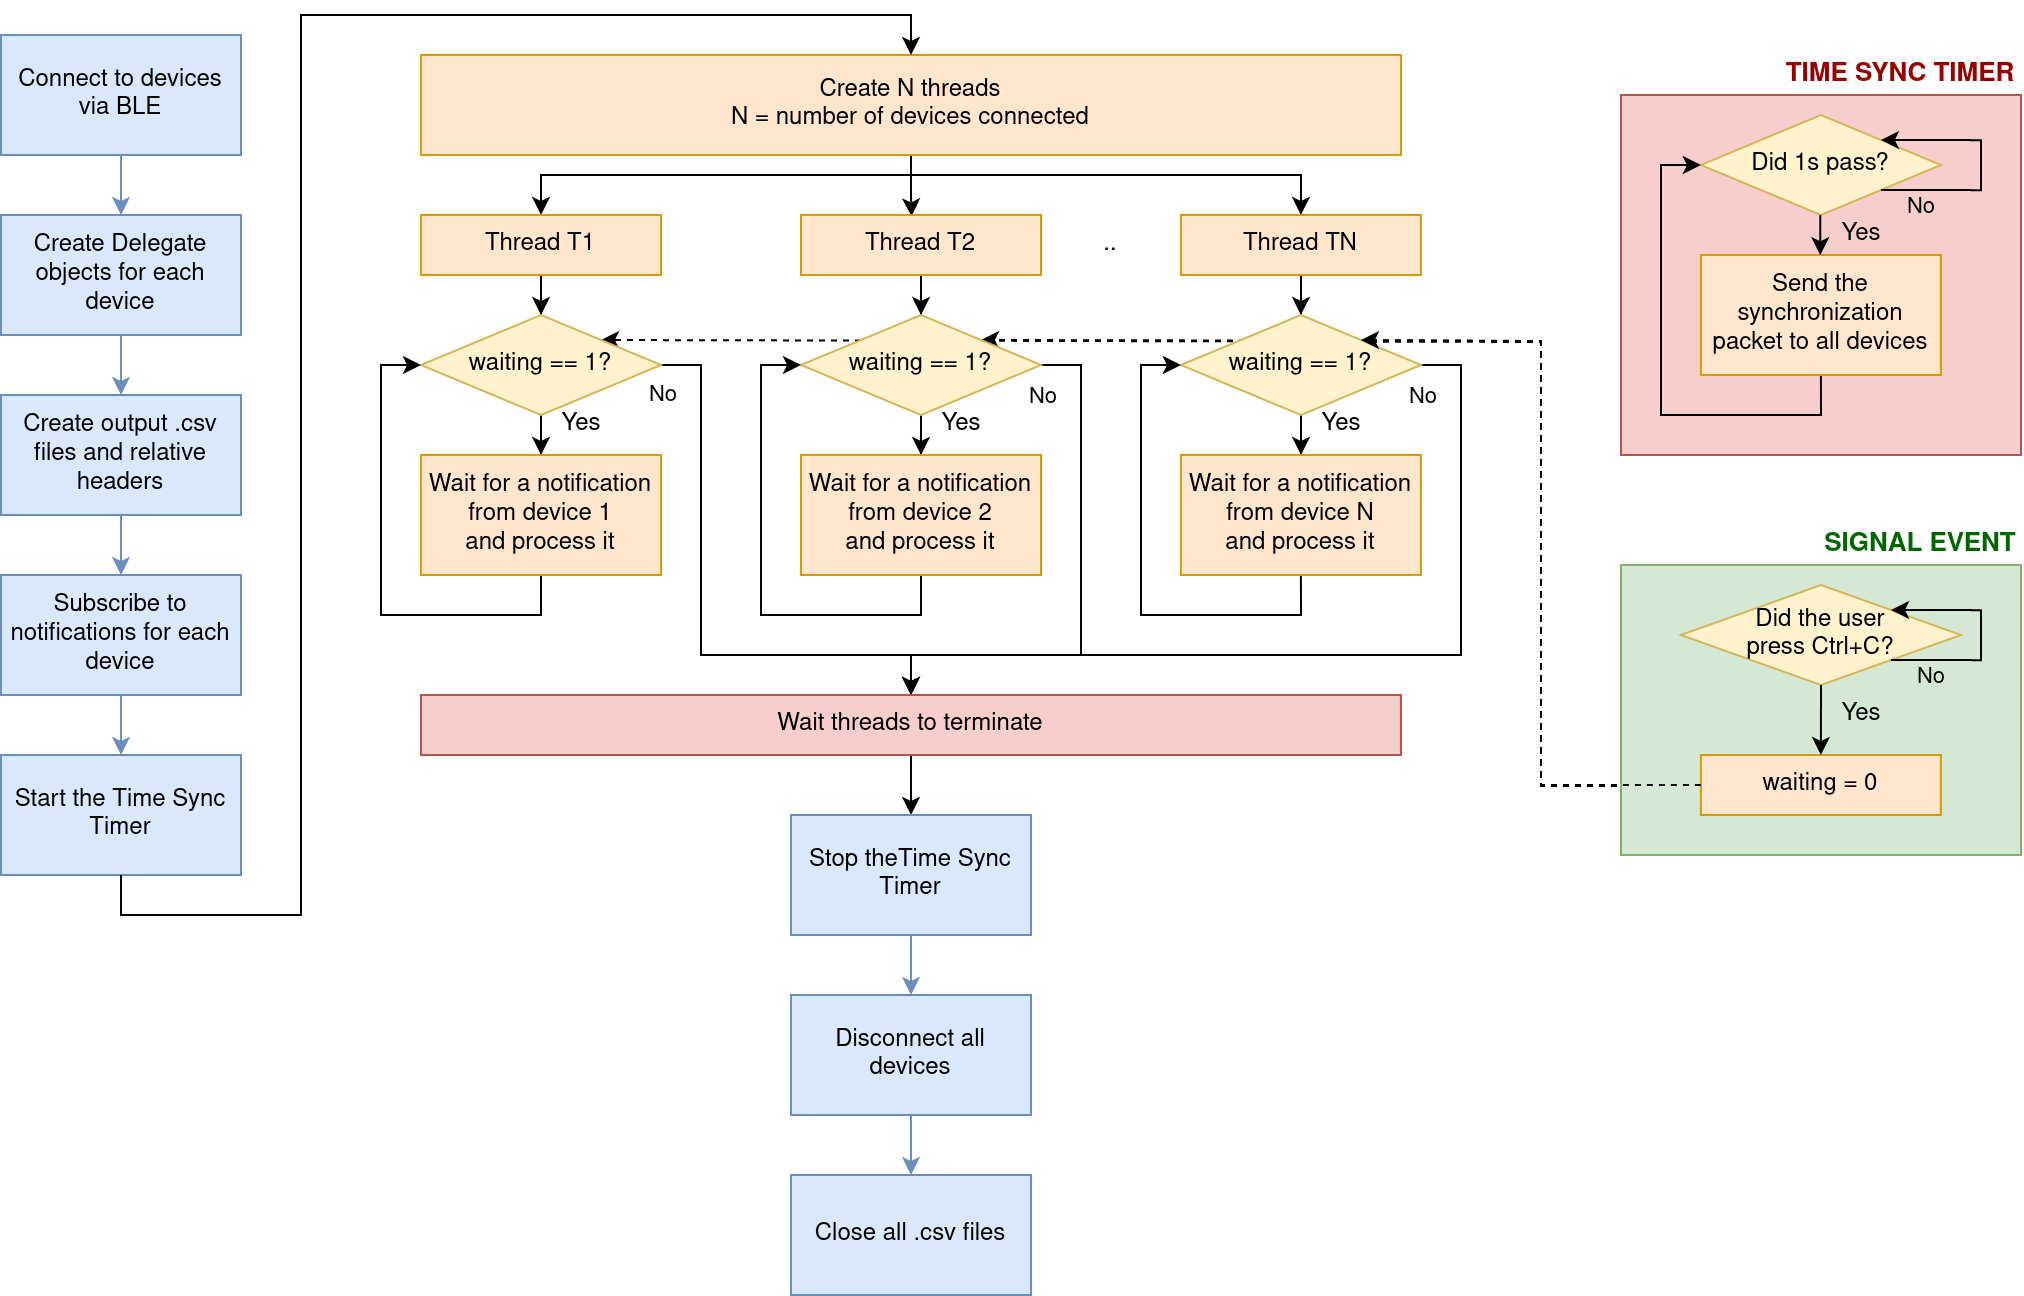
\includegraphics[width=0.85\textwidth]{chap3/figure/Flowchart_st_client(1).png}
        \caption{Flowchart of the client for ST sensor nodes.}
        \label{fig:st-client}
    \end{figure}

\begin{itemize}
    \item \textbf{Connection}. In the first part of the script, I used the \textit{BluePy} library for Python to perform connection to all of the devices. All the information necessary for the connection are reported in a list of dictionaries, each one presenting a) the device name, b) the device MAC address, c) the device type and d) the interface to use for connection. The device type is necessary for the client to understand which features are available (for example, audio dominant frequency is available for the SensorTile.box, only). Also the interface is quite important for our use case, because using multiple Bluetooth adapters leads to better performances (more details in the Results part). It is possible to connect to multiple devices using only one client.

    Once the connection to a device is performed, an object, inherited from the BluePy library, is created for each device. It is called a Delegate, and it contains information for the connection to that device: it is fundamental in our environment, where more than one device is connected. In particular, in this implementation the Delegate holds a) the name of the device; b) the handles used to recognize the type of received data (IMU, environmental, time, audio...) c) the file handles, to write the data into, d) the procedure to be called each time data is received from the device. 

    \item \textbf{Notification handling}. As soon as connection is performed and all Delegates are ready, the clients \textit{subscribes} to the GATT characteristics it is interested to. This procedure varies, based on the type of the device the client it's working with. For example, in the case of the BlueTile (sensing firmware), the client subscribes to IMU sensors, environmental sensors and time synchronization characteristics. 

    After the subscription, each time the sensor node sends data on a particular characteristic, the \textit{handle\_notification} function of the Delegate is called. It will compare the handle with the ones saved in it, understand the type of data received and behave accordingly: in case of sensor data, it is further processed (to use consistent measurement units with MBIENTLAB devices) and written to file, while if it is time synchronization data, the received timestamp and the immediate Unix epoch are saved in the Delegate and used to process successive packets. 

    It is important to add that the BluePy library makes use of the \\\textit{wait\_for\_notification} blocking function, that waits for notification from the precise device it is called from. As we are dealing with more than one device, it is necessary to create different threads, one per node, and then call the function in them using a while condition. As soon as the while condition becomes false, the thread will terminate. 

    \item \textbf{BlueVoice data handling}. In case the ST client is connected to a device of type \textit{bluevoice} (i.e. a BlueTile with the audio streaming firmware), the behaviour is the same of the other ones, but the data received from the node is (of course) treated differently. 
    
    First, timestamps are received from a different GATT characteristics, and should be joined to the audio samples packet. This is performed by using FIFOs lists for both data. 

    Second, data is received compressed, using the ADPCM codec. It means that 16B samples are reduced to 4B samples, that contains only the differences from the previous set of samples. As some packets may get lost, the reconstruction process may not work on the long period: to solve this, the BlueVoice library also sends the so-called sync packets (at lower frequencies). Those contain uncompressed data on which the difference packets can be applied to reconstruct the original signal even if some segment went lost. 
    All this information is processed inside the corresponding functions, \textit{process\_sync} and \textit{process\_audio}, that are released by ST in their GitHub account. 

    \item \textbf{Time Synchronization}. After completing the subscription to all GATT characteristics, the so-called \textit{Repeated Timer} it is created. It is a small Python module making use of the \textit{time} and \textit{threading} libraries to generate a timer that fires at defined intervals, executing a defined function. It is important to note that it has been designed to consider the real interval between firings: the time needed to perform the instructions inside the function will not count. 

    In my implementation, one timer is configured to be fired each second: in the procedure, the synchronization packet is sent to all devices. As explained in Section 3.2, those will respond with a notification, that will be managed accordingly. Other firing intervals can be configured, but smaller ones cause bigger number of packets to be elaborated and exchanged: 1~s is the best tradeoff I found between the number of lost packet and the synchronization accuracy, while 0.5~s caused big percentages of packet loss. 

    \item \textbf{Program termination}. The Ctrl+C signal has been configured to call a procedure that will change the value of the \textit{waiting} variable. That variable is the one that keeps the notification waiting threads alive. In this way, the threads can terminate and join to the main program, that will disconnect from all nodes, close the files and terminate. 

    \item \textbf{BluePy modification}. The BluePy library suffers from a bug that generates exceptions if a GATT characteristic is written while there are multiple threads waiting for notifications. In particular, an object indicating the correct transmission of the packet should be returned to the \textit{writeToCharacteristic} function, that will terminate afterwards. Sometimes that object is received by one of the \textit{wait\_for\_notification} procedures, that are not expecting it, generating an exception. To resolve it, I implemented a workaround, consisting of a) making \textit{wait\_for\_notification} ignore that particular object when received and b) forcing \textit{writeToCharacteristic} to return without waiting for the confirmation object. This does not seem to cause problems in the resynchronization procedure, and we can be confident that the packet is sent by the BLE stack without the need for confirmation. Anyway, this should be considered as only a workaround,  because the problem should be resolved by re-thinking this part of the library (confirmation of the successful transmission is quite important in any case). 
\end{itemize}

\section{Client for MBIENTLAB devices}
I found writing the client for MBIENTLAB MetaMotionS much simpler, as the available APIs and examples are easy to understand and implement. There is no need to implement any time synchronization mechanism, as it's already available by default. Starting from the available Python example, available from the vendor's Github page \cite{metawearsdk}, that is performing the streaming of accelerometer data, I wrote the final version of the script with the following features, with the flowchart represented in Figure \ref{fig:meta-client}.

     \begin{figure}[ht!]
        \centering
        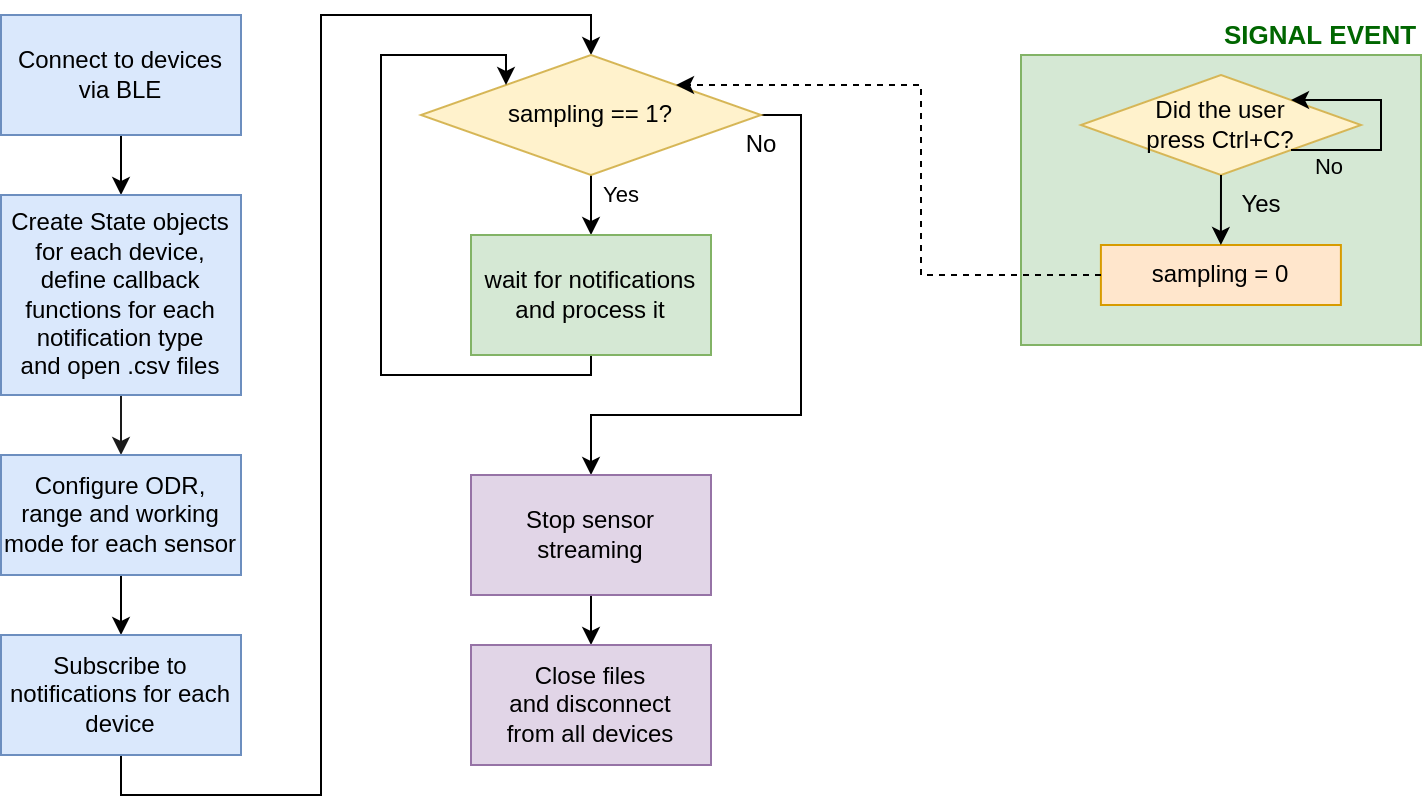
\includegraphics[width=0.85\textwidth]{chap3/figure/Flowchart_meta_client.png}
        \caption{Flowchart of the client for MBIENTLAB sensor nodes.}
        \label{fig:meta-client}
    \end{figure}


\begin{itemize} 
    \item \textbf{Connection}. Also this script support the connection to multiple devices, represented in a list of dictionaries, using multiple Bluetooth adapters. For each sensor node, it is reported a) a name, b) the MAC address of the device and c) the MAC address of the interface to use for connection. The connection is performed by the APIs, so no need to use BluePy (or similar libraries). 

    After the connection, similar to the script for ST nodes, a set of objects, called States, is created. Each of them is responsible for one device, and contains a) the device name, b) the pointers to the functions to be called when data is received and c) the handles of the files in which data is stored.

    The functions are used to take the data from the received packets and save it inside .csv files correctly formatted. To do so, the function \textit{parse\_data}, from the MBIENTLAB APIs is used to get a string containing all data: a regular expression will extract the interesting values from the string and write them into the file. 
    \item \textbf{Configuration}. In the configuration phase, each sensor is configured in its ODR (Output Data Rate), power mode (low power or high accuracy and so on) and range. The sensors configured are IMU (accelerometer, gyroscope, magnetometer), temperature and pressure. This procedure is repeated for each sensor node. At the end, the data collection is started.
    \item \textbf{Data collection stop}. To perform the data collection, I used the Python \textit{sleep} function to make the client wait for notifications. Of course, in the meantime all the received data is processed by the functions pointed inside the State objects. The sleep function, configured to wait for 1s, is repeated until the \textit{sampling} variable remains True: as soon as the Ctrl+C signal makes it become False, the sleep will not be repeated and the Python script will continue its execution. The last lines of code will stop the sampling, reset the sensors, close all the files and print a sum up of the received information. 
\end{itemize}
